\section{一维散射}


\begin{quotation}
``纯科学的发展,人们在更高境界的科学思维所做的努力总会在应用技术领域中得到反映。''\qquad 德布洛意
\end{quotation}

一维``无限深势阱''和``线性谐振子''是束缚态问题,具有分立的能量本征值。
如具有确定动量和能量的粒子由无穷远入射,与``有限高''一维势阱相互作用(或称发生散射),又传播到无穷远处。
由于粒子在全空间都可能出现,所以波函数是无法归一化的,我们只需求出粒子相对几率密度、几率流密度即可。

\subsection{连续条件}

根据波函数的统计解释,要求$\left| \psi  \right|$单值,
不一定要求$\psi $是连续的;粒子数守恒,要求几率流密度连续,
不一定要求$\psi '$是连续的。

由薛定谔方程出发,可讨论$\psi$和$\psi '$的连续性,


\begin{center}
$\psi '' + \frac{{2m}}{{\hbar ^2 }}\left[ {E - V(x)} \right]\psi  = 0$
\end{center}

不同的势$V(x)$表征不同的物理系统,所以$V(x)$决定$\psi '$的连续性。

\begin{center}
$\psi '' =  - \frac{{2m}}{{\hbar ^2 }}\left[ {E - V(x)} \right]\psi $
\end{center}

考虑$x = 0$处, $\psi'$的连续性:$\psi '(\varepsilon ) - \psi '( - \varepsilon ) = \int_{ - \varepsilon }^\varepsilon  {\psi ''dx}  = \int_{ - \varepsilon }^\varepsilon  { - \frac{{2m}}{{\hbar ^2 }}\left[ {E - V(x)} \right]\psi dx} $

定态薛定谔,能量为确定值,$\psi$有限,所以:$\int_{ - \varepsilon }^\varepsilon  {E\psi dx \to 0} $

考虑积分:$\int_{ - \varepsilon }^\varepsilon  {V(x)\psi dx} $,

如$V(x)$连续, $\int_{ - \varepsilon }^\varepsilon  {V(x)\psi dx}
\to 0$, $\psi '$连续。

如$V(x)$不连续,跃变值有限,$\int_{ - \varepsilon }^\varepsilon  {V(x)\psi dx}  = V_0 \psi (x_0 )2\varepsilon  \to 0$,$\psi '$连续。

如$V(x)$不连续,跃变值无限,$\int_{ - \varepsilon }^\varepsilon  {V(x)\psi dx} $发散,$\psi '$不连续(无限高势阱)。

如$V(x)$在$\left( { - \varepsilon ,\varepsilon } \right)$含奇异点($\delta $函数),$\int_{ - \varepsilon }^\varepsilon  {V(x)\psi dx}  = \int_{ - \varepsilon }^\varepsilon  {V_0 \delta (x)\psi dx = V_0 \psi (x_0 )} $,$\psi '$不连续;($\delta$势阱)

考虑波函数在$x=0$处的连续性:

\begin{center}
$\psi (\varepsilon ) - \psi ( - \varepsilon ) = \int_{ - \varepsilon }^\varepsilon  {\psi 'dx} $
\end{center}

如$\psi '$连续,$\psi (\varepsilon ) - \psi ( - \varepsilon ) \to 0$,即:$\psi$连续;

如$\psi '$不连续,$\psi '$跃变为有限值,$\psi (\varepsilon ) - \psi ( - \varepsilon ) = \int_{ - \varepsilon }^\varepsilon  {\psi 'dx}  \to 0$,即$\psi$连续;

如$\psi '$不连续,$\psi '$跃变为无限或含奇异性,$\psi$不连续;
在考虑波函数连续条件时,要时刻注意回到原始的物理条件,即:
``势函数''、``波函数的统计解释''、``连续性方程\ref{continue eq}''和``薛定谔方程\ref{schrodinger eq}''去考虑,
而不能根据经验想当然。

\subsection{台阶势}

\index{Step potential: 台阶势}

\begin{figure}[h]
\begin{center}
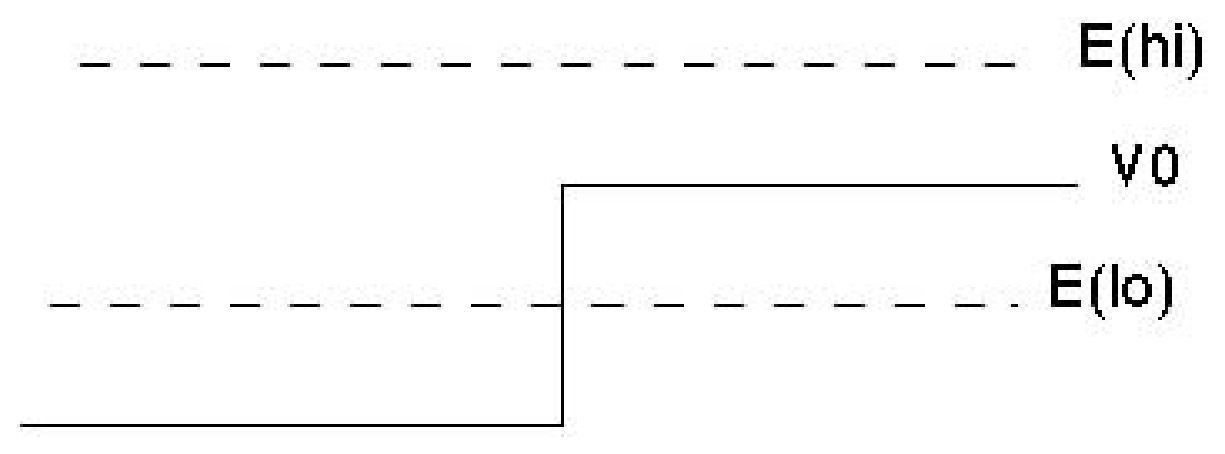
\includegraphics[clip,width=8cm]{1DProblem/11-1.ps}
\caption{台阶势,势垒高度为$V_0$}
\end{center}
\end{figure}

\textbf{首先讨论经典粒子在台阶势场中的运动:}

若$E < V_0 $,粒子被全部反射($R=1$);若$E > V_0 $,粒子全部透射($T=1$),但粒子运动速度会变小。($v = \sqrt {\frac{{2(E - V_0 )}}{m}}$)

\textbf{量子情形:}

(1)$E < V_0 $:

\begin{figure}[h]
\begin{center}
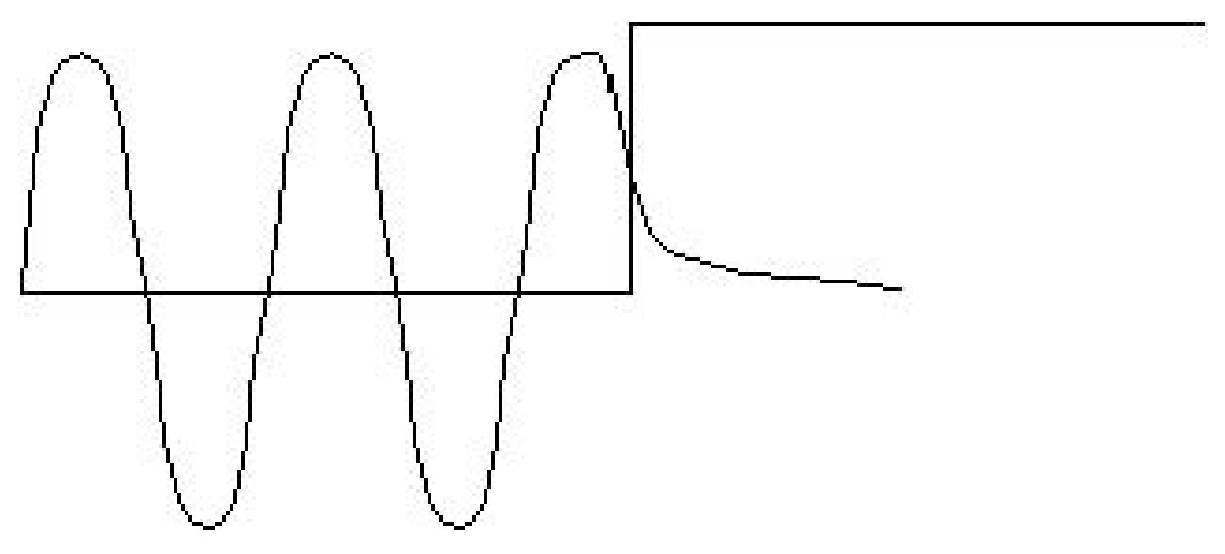
\includegraphics[clip,width=8cm]{1DProblem/11-2.ps}
\caption{量子情形,$E < V_0$波函数的分布}
\end{center}
\end{figure}

对波函数的解作定性分析:左侧为正弦型振荡,右侧为指数型衰减,波无法向前传播,所以透射系数为0,对应全部反射,类似光学中的全反射现象。
但粒子在能量E小于势垒高度时仍能出现。在全反射现象中,电磁场在折射介质中也有分布,但呈指数型衰减,所以不能传播,对应透射系数也是0。

对$x>0$,$x<0$分别列出薛定谔方程:

\begin{center}
$\left\{ \begin{array}{l}
  - \frac{{\hbar ^2 }}{{2m}}\frac{{d^2 \psi }}{{dx^2 }} = E\psi ,x < 0 \\
  - \frac{{\hbar ^2 }}{{2m}}\frac{{d^2 \psi }}{{dx^2 }} = \left( {E - V{}_0} \right)\psi ,x > 0 \\
 \end{array} \right.$
\end{center}

可化简为:

\begin{center}
$\left\{ \begin{array}{l}
 \psi '' + k^2 \psi  = 0,k^2  = \frac{{2mE}}{{\hbar ^2 }} \\
 \psi '' - \beta ^2 \psi  = 0,\beta ^2  = \frac{{2m\left( {V_0  - E} \right)}}{{\hbar ^2 }} \\
 \end{array} \right.$
\end{center}

波函数的解可写为:

\begin{center}
$\left\{ \begin{array}{l}
 \psi _I  = Ae^{ikx}  + Be^{ - ikx}  \\
 \psi _{II}  = Ce^{ - \beta x}  \\
 \end{array} \right.$
\end{center}

其中$A$,$B$,$C$是待定系数,可通过边界条件将它们确定。

由于势垒是有限高的,所以波函数及其导数在$x=0$处连续:

\begin{center}
$\left\{ \begin{array}{l}
 A + B = C \\
 A - B = i\frac{\beta }{k}C \\
 \end{array} \right.$
\end{center}

由此可得:

\begin{center}
$\left\{ \begin{array}{l}
 2B = C\left( {1 - i\frac{\beta }{k}} \right) \\
 2A = C\left( {1 + i\frac{\beta }{k}} \right) \\
 \end{array} \right.$
\end{center}

化简后,可得:

\begin{center}
$\left\{ \begin{array}{l}
 C = \frac{{2A}}{{1 + i\frac{\beta }{k}}} \\
 B = \left( {\frac{A}{{1 + i\frac{\beta }{k}}}} \right)\left( {1 - i\frac{\beta }{k}} \right) = \frac{{A\left( {1 - i{\textstyle{\beta  \over k}}} \right)^2 }}{{1 + \left( {{\textstyle{\beta  \over k}}} \right)^2 }} \\
 \end{array} \right.$
\end{center}

入射粒子流密度,反射粒子流密度可表示为:

\begin{center}
$\left\{ \begin{array}{l}
 J_{in}  = \frac{{i\hbar }}{{2m}}\left( {\psi \nabla \psi ^*  - \psi ^* \nabla \psi } \right) = \frac{{\hbar k}}{m}\left| A \right|^2  \\
 J_{re}  =  - \frac{{\hbar k}}{m}\left| B \right|^2  \\
 \end{array} \right.$
\end{center}

由于:$\left| B \right|^2  = \left| {\frac{{1 - 2i{\textstyle{\beta  \over k}} - \left( {{\textstyle{\beta  \over k}}} \right)^2 }}{{1 + \left( {{\textstyle{\beta  \over k}}} \right)^2 }}} \right|^2 \left| A \right|^2  = \frac{{\left[ {1 - \left( {{\textstyle{\beta  \over k}}} \right)^2 } \right]^2  + 4\left( {{\textstyle{\beta  \over k}}} \right)^2 }}{{\left[ {1 + \left( {{\textstyle{\beta  \over k}}} \right)^2 } \right]^2 }}\left| A \right|^2  = \frac{{\left[ {1 + \left( {{\textstyle{\beta  \over k}}} \right)^2 } \right]^2 }}{{\left[ {1 + \left( {{\textstyle{\beta  \over k}}} \right)^2 } \right]^2 }}\left| A \right|^2  = \left| A \right|^2 $

所以,反射系数:$R = \frac{{J_{re} }}{{J_{in} }} = 1$,透射系数:$T = 1 - R = 0$

(2)$E > V_0 $:

定态薛定谔方程可写为:

\begin{center}
$\left\{ \begin{array}{l}
  - \frac{{\hbar ^2 }}{{2m}}\frac{{d^2 \psi }}{{dx^2 }} = E\psi ,x < 0 \\
  - \frac{{\hbar ^2 }}{{2m}}\frac{{d^2 \psi }}{{dx^2 }} + V_0 \psi  = E\psi ,x > 0 \\
 \end{array} \right.$
\end{center}

可化简为:

\begin{center}
$\left\{ \begin{array}{l}
 \psi '' + k_1 ^2 \psi  = 0,k_1 ^2  = \frac{{2mE}}{{\hbar ^2 }},x < 0 \\
 \psi '' + k_2 ^2 \psi  = 0,k_2 ^2  = \frac{{2m(E - V_0 )}}{{\hbar ^2 }},x > 0 \\
 \end{array} \right.$
\end{center}

波函数可写为:

\begin{center}
$\left\{ \begin{array}{l}
 \psi _I  = Ae^{ik_1 x}  + Be^{ - ik_1 x}  \\
 \psi _{II}  = Ce^{ik_2 x}  \\
 \end{array} \right.$
\end{center}

在$x=0$处,列出波函数及其导数连续的边界条件:

\begin{center}
$\left\{ \begin{array}{l}
 A + B = C \\
 ik_1 A - ik_1 B = ik_2 C \Rightarrow k_1 (A - B) = k{}_2C \\
 \end{array} \right.$
\end{center}

所以:$k_2 \left( {A + B} \right) - k_1 \left( {A - B} \right) = 0 \Rightarrow A\left( {k_1  - k_2 } \right) = B\left( {k_1  + k_2 } \right)$

所以:$\frac{B}{A} = \frac{{k_1  - k_2 }}{{k_1  + k_2 }}$,

反射系数:$R = \frac{{\left| B \right|^2 }}{{\left| A \right|^2 }} = \left( {\frac{{k_1  - k_2 }}{{k_1  + k_2 }}} \right)^2 $

透射系数:$T = 1 - R = \frac{{4k_1 k_2 }}{{\left( {k_1  + k_2 } \right)^2 }}$

由边界条件:$A+B=C$,可解出:$A + A\left( {\frac{{k_1  - k_2 }}{{k_1  + k_2 }}} \right) = C \Rightarrow A\left( {\frac{{2k_1 }}{{k_1  + k_2 }}} \right) = C$

所以:$\frac{C}{A} = \frac{{2k_1 }}{{k_1  + k_2 }}$

\textbf{思考题:}为什么:$T \ne \left| {\frac{C}{A}} \right|^2  = \frac{{4k_1 ^2 }}{{\left( {k_1  + k_2 } \right)^2 }}$

\subsection{势垒穿透}

\index{Tunneling: 隧穿}

假设质量为$m$的粒子在势场$V(x)$中运动。

\begin{center}
$V(x) = \left\{ \begin{array}{l}
 V_0 ,x \in \left( {0,a} \right) \\
 0,{\rm{others}} \\
 \end{array} \right.$
\end{center}

\begin{figure}[h]
\begin{center}
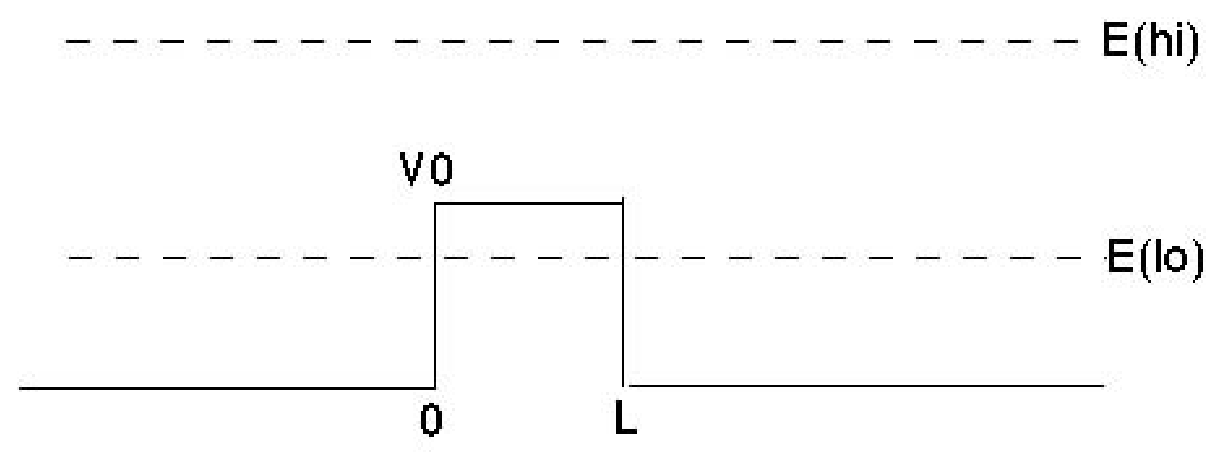
\includegraphics[clip,width=10cm]{1DProblem/11-3.ps}
\caption{粒子在高度为$V_0$的势垒中运动}
\end{center}
\end{figure}

若$E<V_0$,波函数可写为:

\begin{center}
$\psi \left( x \right) = \left\{ \begin{array}{l}
 A_1 e^{ikx}  + A_2 e^{ - ikx} ,x < 0 \\
 B_1 e^{\alpha x}  + B_2 e^{ - \alpha x} ,x \in \left[ {0,a} \right] \\
 Ce^{ikx} ,x > a \\
 \end{array} \right.$
\end{center}

其中:$k^2  = \frac{{2mE}}{{\hbar ^2 }},\alpha ^2  = \frac{{2m\left( {V_0  - E} \right)}}{{\hbar ^2 }}$

粒子几率流密度可表示为:

\begin{center}
$\begin{array}{l}
 J_{in}  = \frac{{i\hbar }}{{2m}}\left( {\psi \nabla \psi ^*  - \psi ^* \nabla \psi } \right) = \frac{{\hbar k}}{m}\left| {A_1 } \right|^2  = v\left| {A_1 } \right|^2  \\
 J_{re}  =  - \frac{{\hbar k}}{m}\left| {A_2 } \right|^2  =  - v\left| {A_2 } \right|^2  \\
 J_{out}  = \frac{{\hbar k}}{m}\left| C \right|^2  = v\left| C \right|^2  \\
 \end{array}$
\end{center}

\begin{figure}[h]
\begin{center}
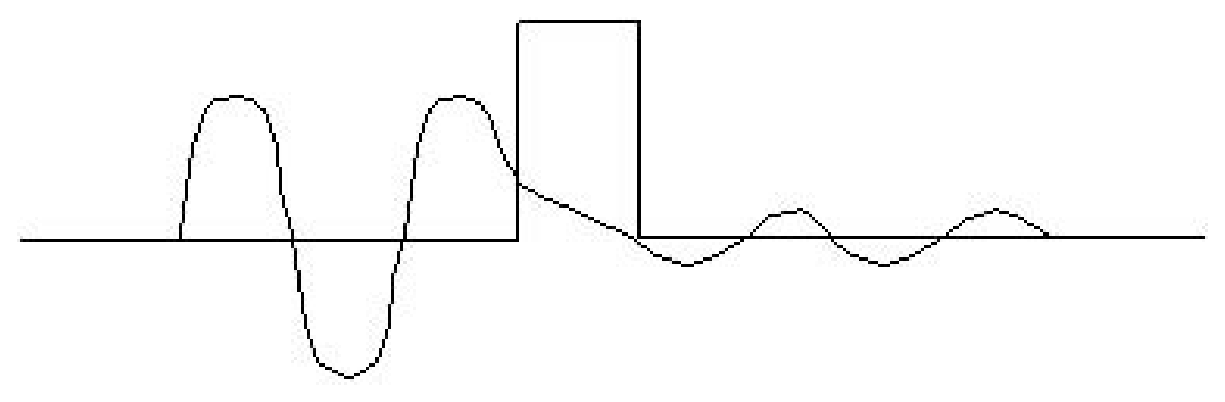
\includegraphics[clip,width=10cm]{1DProblem/11-4.ps}
\caption{粒子在高度为$V_0$的势垒中运动:波函数}
\end{center}
\end{figure}

对$x=0$和$x=a$,分别列出波函数满足的边界条件:

$x=0$时,

\begin{center}
$\left\{ \begin{array}{l}
 A_1  + A_2  = B_1  + B_2  \\
 ikA_1  - ikA_2  = \alpha B_1  - \alpha B_2 ,ik\left( {A_1  - A_2 } \right) = \alpha \left( {B_1  - B_2 } \right) \\
 \end{array} \right.$
\end{center}

$x=a$时,

\begin{center}
$\left\{ \begin{array}{l}
 B_1 e^{\alpha a}  + B_2 e^{ - \alpha a}  = Ce^{ika}  \\
 \alpha B_1 e^{\alpha a}  - \alpha B_2 e^{ - \alpha a}  = ikCe^{ika} ,\alpha \left( {B_1 e^{\alpha a}  - \alpha B_2 e^{ - \alpha a} } \right) = ikCe^{ika}  \\
 \end{array} \right.$
\end{center}

5个未知量($A_1$, $A_2$, $B_1$, $B_2$, $C$),4个方程,方程组联立解得:

\begin{center}
$\left\{ \begin{array}{l}
 \frac{C}{{A_1 }} = \frac{{2ik\alpha e^{ - ika} }}{{\left( {k^2  - \alpha ^2 } \right)sh\left( {\alpha a} \right) + 2ik\alpha ch\left( {\alpha a} \right)}} \\
 \frac{{A_2 }}{{A_1 }} = \frac{{\left( {k^2  + \alpha ^2 } \right)sh\left( {\alpha a} \right)}}{{\left( {k^2  - \alpha ^2 } \right)sh\left( {\alpha a} \right) + 2ik\alpha ch\left( {\alpha a} \right)}} \\
 \end{array} \right.$
\end{center}


反射系数与透射系数为:

\begin{center}
$\left\{ \begin{array}{l}
 T = \left| {\frac{C}{{A_1 }}} \right|^2  = \frac{{4k^2 \alpha ^2 }}{{\left( {k^2  - \alpha ^2 } \right)^2 \sinh ^2 \left( {\alpha a} \right) + 4k^2 \alpha ^2 \cosh ^2 \left( {\alpha a} \right)}} = \frac{{4k^2 \alpha ^2 }}{{\left( {k^2  + \alpha ^2 } \right)^2 \sinh ^2 \left( {\alpha a} \right) + 4k^2 \alpha ^2 }} \\
 R = \left| {\frac{{A_2 }}{{A_1 }}} \right| = 1 - T = \frac{{\left( {k^2  + \alpha ^2 } \right)^2 \sinh ^2 \left( {\alpha a} \right)}}{{\left( {k^2  + \alpha ^2 } \right)^2 \sinh ^2 \left( {\alpha a} \right) + 4k^2 \alpha ^2 }} \\
 \end{array} \right.$
\end{center}

若$E>V_0$,我们也可类似地求出反射和透射系数。

\subsection{WKB近似}

\index{WKB approximation: WKB近似}

在势垒的反射、透射系数公式中,如果:$\alpha a = \sqrt {\frac{{2m\left( {V_0  - E} \right)}}{{\hbar ^2 }}} a \gg 1$,透射系数可近似表示为:$T = T_0 \exp \left( { - {\textstyle{2 \over \hbar }}\sqrt {2m\left( {V_0  - E} \right)}  \cdot a} \right)$


对任意形状势函数: $V(x)>E$

\begin{equation}\label{11-1}
T = T_0 e^{ - {\textstyle{2 \over \hbar }}\sqrt {2m\left( {V(a) - E} \right)} dx}  \cdot e^{ - {\textstyle{2 \over \hbar }}\sqrt {2m\left( {V(a + dx) - E} \right)} dx} ... = T_0 e^{ - {\textstyle{2 \over \hbar }}\int_a^b {\sqrt {2m\left( {V(x) - E} \right)} dx} }
\end{equation}

这就是WKB近似,也叫准经典近似,
即$\hbar  \to 0$极限下的解
\footnote{假设波函数:$\psi  = \exp \left( {\frac{{iS}}{\hbar }} \right)$,是薛定谔方程:$ - \frac{{\hbar ^2 }}{{2m}}\frac{{d^2 }}{{dx^2 }}\psi  + V(x)\psi  = E\psi $的解

波函数一阶导数:$\frac{{d\psi }}{{dx}} = \frac{i}{\hbar }\psi \frac{{dS}}{{dx}}$

二阶导数:$\frac{{d^2 }}{{dx^2 }}\psi  = \frac{d}{{dx}}\left( {\frac{i}{\hbar }\psi \frac{{dS}}{{dx}}} \right) = \frac{i}{\hbar }\left( {\frac{{d\psi }}{{dx}}\frac{{dS}}{{dx}} + \psi \frac{{d^2 S}}{{dx^2 }}} \right) = \left( {\frac{i}{\hbar }} \right)^2 \left( {\frac{{dS}}{{dx}}} \right)^2 \psi  + \frac{i}{\hbar }\frac{{d^2 S}}{{dx^2 }}\psi $

代入薛定谔方程:$\frac{1}{{2m}}\left( {\frac{{dS}}{{dx}}} \right)^2  + \frac{\hbar }{i}\frac{1}{{2m}}\frac{{d^2 S}}{{dx^2 }} = E - V(x)$,在$\hbar  \to 0$,$E > V\left( x \right)$条件下:

$\frac{1}{{2m}}\left( {\frac{{dS}}{{dx}}} \right)^2  = E - V(x)$,即:$\left( {\frac{{dS}}{{dx}}} \right)^2  = 2m\left( {E - V(x)} \right)$

所以:$\frac{{dS}}{{dx}} = \sqrt {2m\left( {E - V(x)} \right)} $,对$x$积分:$S = \int_x {\sqrt {2m\left( {E - V(x)} \right)} dx}  + {\rm{Const}}$

透射系数:$T \sim v\left| {\psi ^2 } \right| \sim T_0 \exp \left( { - {\textstyle{2 \over \hbar }}\int_x {\sqrt {2m\left( {E - V(x)} \right)} dx} } \right)$,即WKB近似\ref{11-1}。
}。

\subsection{扫描隧道显微术}

\begin{figure}[h]
\begin{center}
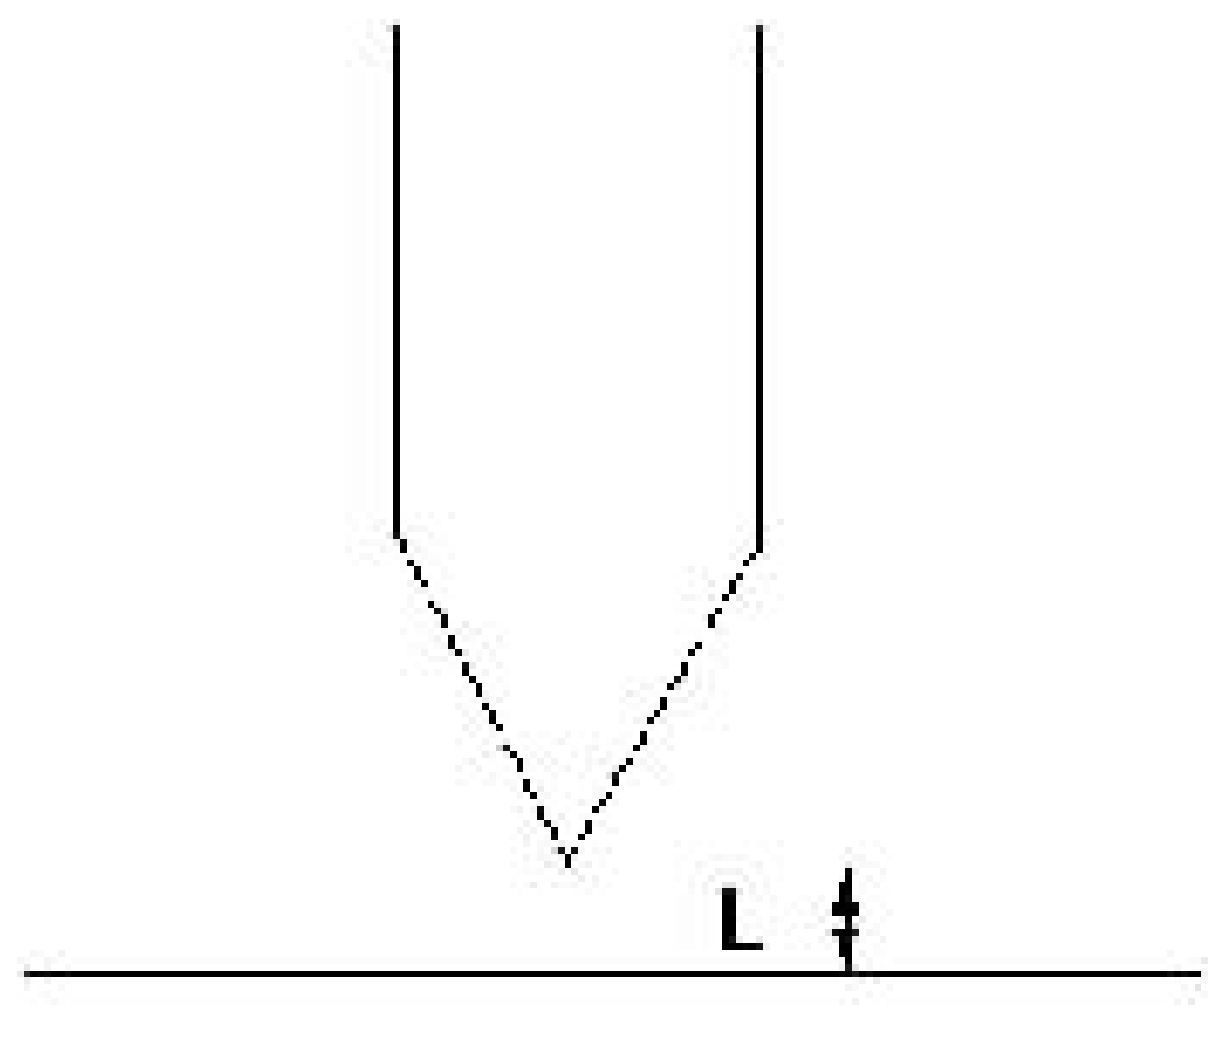
\includegraphics[clip,width=6cm]{1DProblem/11-5.ps}
\caption{扫描隧道显微镜示意}
\end{center}
\end{figure}

\index{STM, scanning tunneling microscope, 扫描隧道显微术}

扫描隧道显微术(STM, scanning tunneling microscope)是一种新型表面分析仪器,其原理如图,
量子系统可看作是宽度为$L$的势垒,隧穿电流(正比于粒子流密度)随间距$L$的变化而变化十分敏锐,
测出透射电流的变化,即可知道固体表面的``形貌''(相当于在测量固体表面的``等高线'')。
扫描隧道显微术是1981年由宾尼(G. Binnig)和罗拉尔(H. Rohrer)\footnote{宾尼和罗拉尔因此获得了1986年诺贝尔物理奖。}发明的,可获得$0.01nm$的纵向分辨率,它不仅可以应用于真空环境,
而且可用于大气环境(大气STM技术)和液体环境(电解质STM技术)下。近10多年来,扫描隧道显微术发展非常迅速,
还发展出原子力显微术(AFM, atomic force microscopy)和磁力显微术(MFM, magnetic force microscopy)。目前STM,AFM,MFM等都已发展为商品。

实验物理学家最早是使用X射线衍射固体表面的,
德布洛意在1945年巴黎``表面状态研究''会议闭幕式上的讲演中曾讲过威尼斯总督的故事,以赞叹纯粹科学在技术中的应用。
``威尼斯的总督从未离开他统治的城市。
由于某个机会使他来到凡尔塞路易十四的宫廷。
当路易问他在凡尔塞最繁荣昌盛的此时此刻最使他欣赏的是什么,
他回答道:`我在这个城市里发现了我自己。'''


要理解量子力学的真正意义,我们就必须了解量子力学在现代技术中的应用。



\subsection*{阅读与思考}

\begin{itemize}

\item \textbf{变质量量子系统}\footnote{参考: 柯善哲 等编《量子力学朝花夕拾(第二辑)》, pp38 }:
电子在半导体量子井中传播,能量为$E$,在I,III区中电子有效质量为$m_1$,
势垒高度为$0$;在II区中电子有效质量为$m_2$,势垒高度为$V$。
列出这个量子力学问题的薛定谔方程及边界条件,并求解透射系数。

\begin{figure}[h]
\begin{center}
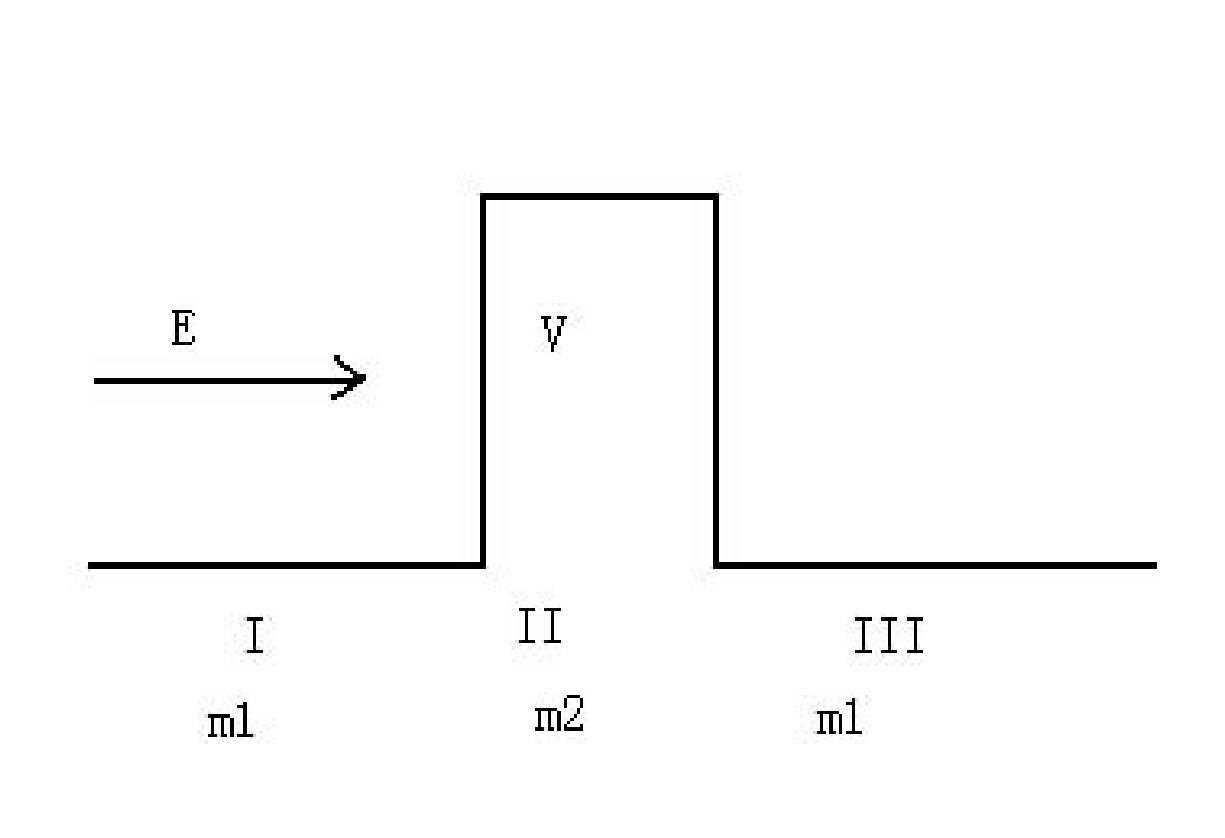
\includegraphics[clip,width=8cm]{1DProblem/quantum_well.ps}
\caption{半导体量子井}
\end{center}
\end{figure}


\index{Topological insulator: 拓扑绝缘体}

\item \textbf{拓扑绝缘体:} 拓扑绝缘体(topological insulator)是一种新的量子物质态,
这种物质的体电子态是绝缘体(有能隙), 而表面电子态是无能隙的金属态。
拓扑绝缘体的表面金属态完全由材料的体电子态的拓扑结构决定,
由对称性决定, 与表面的具体结构无关, 因此表面金属态的存在非常稳定,
基本不受杂质与无序的影响。

拓扑绝缘体的基本性质是由``量子力学''和 ``相对论''共同作用的结果,
由于``自旋-轨道相互作用'',
在表面上会产生由时间反演对称性保护的无能隙的自旋分辨的表面电子态。这种表面态形成一种无有效质量的二维电子气,
需要用狄拉克方程来描述。

最近的一项研究使用扫描隧道显微术(STM)测量了锑(antimony)的表面电子态密度,
实验表明尽管存在表面缺陷, 处在拓扑表面态的电子仍有高的电导率。



\textbf{新闻}: ``Topological electrons reach the next step'',
\url{http://physicsworld.com/cws/article/news/43203}

\textbf{论文}: ``Transmission of topological surface states through
surface barriers'', \url{http://cn.arxiv.org/abs/1007.2445}


这里有相当多名词是陌生和奇妙的, 等本课程结束的时候再回过头来读读,
看看有没有明白些。



\end{itemize}
